\title{COM S 352 Homework 2}
\author{Alec Meyer}

\date{\today}

\documentclass[11pt]{article}
\usepackage{changepage}
\usepackage{graphicx}
\usepackage{amsmath}
\graphicspath{ {./images/} }
\newcommand\tab[1][1cm]{\hspace*{#1}}
\usepackage{amssymb}


\begin{document}
\maketitle


\section*{Question 1}
    First the operating system saves all data then transfers 
    control the the kernal. The kernel saves the context of 
    the old proccess in its PCB and then grabs the new process 
    and loads the saved data into the new process. Finally the 
    OS transfers control back to user mode.
\section*{Question 2}
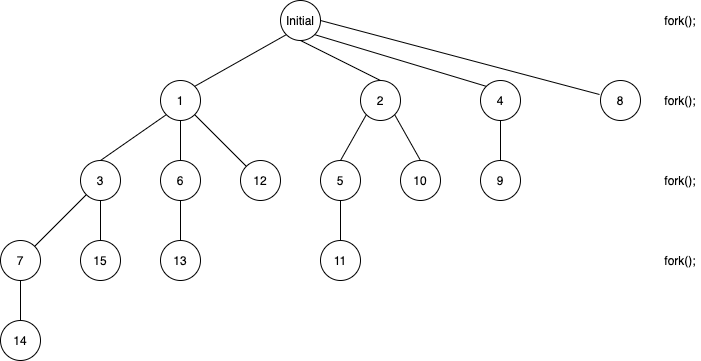
\includegraphics[scale=0.52]{COMS352HW2Q2}
16 total processes created 

\newpage
\section*{Question 3}
    The program executes, then runs into the \emph{fork()} function,
    where it creates a child process. This child process will enter 
    the \emph{else if} statement because its pid is 0 then it will
    hit the \emph{exec()} function. The \emph{exec()} function replaces
    the childs memory space with a new program, in this case it is
    \emph{ls}. Now that the child no longer exsists it will not reach 
    the line, \emph{printf("LINE J")}. However, if the \emph{exec()}
    function results in an error and memory is not replaced the
    child process will run the line \emph{printf("LINE J")}.
\section*{Question 4}
A: 0    \, \quad \qquad  //child\\
B: 2606 \qquad //child\\
C: 2606 \qquad //parent\\
D: 2603 \qquad //parent\\

\newpage
\section*{Question 5}
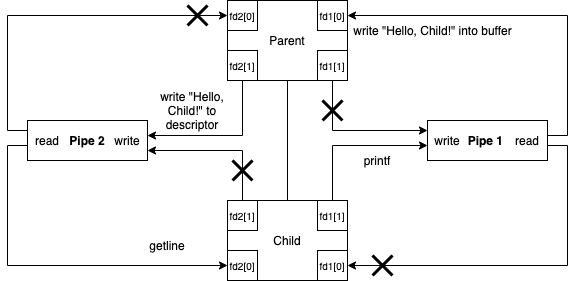
\includegraphics[scale=0.6]{COMS352HW2Q5.png}\\
The program will start by initializing its pipes and forks, creating
a Parent (2603), Child (2606) and two pipes; fd1, fd2.\\
1. The Child calls \emph{dup2(fd[1], 1)} which duplicates the file descriptor
and redirects it to STDOUT\\
2. The Child calls \emph{dup2(fd[0], 0)} which duplicates the file descriptor
and redirects it to STDIN\\
3. The Child calls \emph{execlp("cat", "cat", NULL)} which echos STDIN to 
STDOUT\\
4. The Child process terminates. \\
Described above creates a path from pipe 1 all the way to pipe 2. 
This path can be seen on the diagram represented by the red bold arrows.
This path will allow the Parent to write to pipe 2 and read the message
from pipe 1. Now that the parent has read the message it is stored into
the buffer which prints "Hello, Child!".

\newpage
\section*{Question 6}
    $\delta / (\delta + \sigma)$\\\\
    System A:\\
    $\delta$ = 20ms\\
    $\sigma$ = 1ms\\\\
    $20 / (20 + 1)$\\
    = 95.24\%\\\\
    System B:\\
    $\delta$ = 15ms\\
    $\sigma$ = 1ms\\\\
    $15 / (15 + 1)$\\
    =93.75\%\\
    The system with a slice of 20ms will be more efficient by 1.49\%

\section*{Question 7}
\begin{enumerate}
    \item \textbf{Running to Waiting}\\
        During an I/O or event wait, The process is going to enter a 
        waiting state because it is waiting for I/O input/output.
    \item \textbf{Waiting to Ready}\\
        After waiting for an I/O response (completion) it 
        will move to a ready state where it waits for 
        reassignment.
    \item \textbf{Running to Ready}\\
        The transition from running to ready will 
        occur when an interrupt is triggered. 
\end{enumerate}
\end{document}
